\documentclass{article}
\usepackage[a4paper, margin=2.5cm]{geometry}
\usepackage{polski, graphicx, float, siunitx}
\setcounter{secnumdepth}{0}

\begin{document}
\subsection{Przetwornica 12V na 5V}
\subsubsection{Zastosowanie}

Z powodu dodania paska LED, który wymaga zasilania 5V oraz prądów rzędu 2A, zdecydowano się na samodzielne zaprojektowanie przetwornicy, gdyż gotowe moduły
psułyby estetykę zegara. Nie zastosowano również stabilizatora liniowego, gdyż było by to nieefektywne i wymagało dodatkowego radiatora.

Zdecydowano się na przetwornicę impulsową, która jest znacznie bardziej efektywna. Dzięki temu również można było zminimalizować straty mocy na zasilaniu linii 3.3V, ponieważ
można było zastosowac LDO zamiast stabilizatora liniowego z 12V na 3.3V.
\subsubsection{Wybór układu scalonego}

Zdecydowano się na układ TPS563219ADDFR produkcji Texas Instruments, który jest przetwornicą impulsową z wbudowanym tranzystorem mocy oraz zapewniajacym prąd wyjściowy do 3A przy 
napięciu wyjściowym do 7V. Układ jest też w obudowie na tyle dużej, by móc go polutować ręcznie. Układ posiada soft-start oraz wyjście power good (potwierdzające start przetwornicy), co nie jest potrzebne w tym zastosowaniu, tak samo 
nie jest to najmniejszy układ, ale zapewnia to łatwość montażu co jest ważne w tym przypadku.

\subsubsection{Założenia projektowe}
% obliczenia szacowanego prądu ledów i reszty komponentów
\begin{itemize}
    \item Napięcie wejściowe: 12V
    \item Napięcie wyjściowe: 5V
    \item Prąd wyjściowy: 2A
    \item 50mV tętnienia napięcia wyjściowego
\end{itemize}

\subsubsection{Dobór komponentów}
Dobór komponentów wykonano na podstawie sugerowanych wartości z noty katalogowej układu TPS563219ADDFR.

\begin{figure}[H]
    \centering
    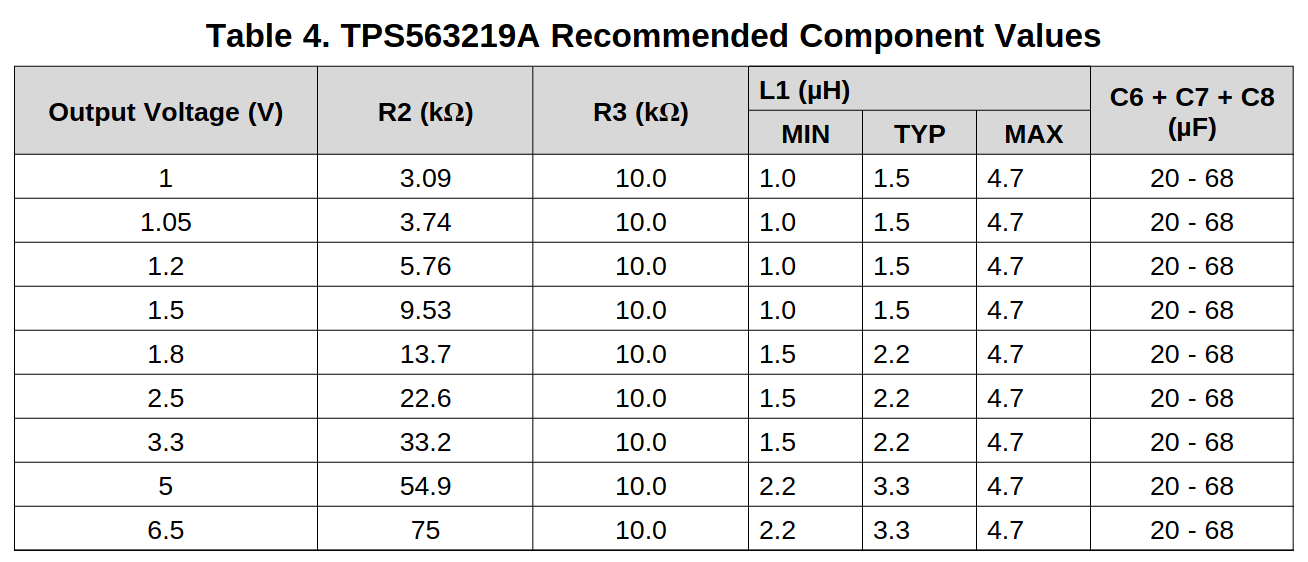
\includegraphics[width=0.8\textwidth]{conv-table.png}
    \caption{Tabela doboru komponentów z noty katalogowej}
\end{figure}

Na podstawie tabeli dobrano następujące wartości komponentów:
\begin{itemize}
    \item C1: 22uF 10V
    \item C29: 22uF 10V
    \item L1: 2.2uH 9.2A 14.5m$\Omega$
    \item R1: 56k$\Omega$
    \item R2: 10k$\Omega$
\end{itemize}

Kondensator podpięty pod pin SS(soft start) oraz kondensator podpięty pod pin VBST, został skopiowany z układu z noty katalogowej, gdyż nie jest to krytyczny element i nie ma potrzeby doboru wartości pod 
kątem zastosowania w zegarze.

Zdecydowano się na użycie kondensatorów ceramicznych, gdyż są one mniejsze i mają lepszy ESR niż elektrolityczne, co ma znaczenie przy przetwornicach impulsowych,
gdzie mamy wyższe częstotliwości przełączania, więc ESR kondensatora ma większe znaczenie, przy zbyt dużym ESR kondensatora, może on się nagrzewać, co prowadzi do jego uszkodzenia.
Kondensatory ceramiczne natomiast cechują się tak małym ESR, że producent nie podaje tej wartości w notach katalogowych, gdyż jest ona zbyt mała by miała znaczenie.

Cewka dobrano biorąc pod uwagę jest stosunek oporu do ceny, zdecydowano się na cewkę o oporze 14.5m$\Omega$, 
gdyż jest to najniższa wartość jako udało się znaleźć w sklepach elektronicznych w sensownej cenie i dość małej obudowie.

Dodano również kondensator filtrujący 100nF na pinie VCC, by zredukować szumy z linii zasilania.

\subsubsection{Schemat}
\begin{figure}[H]
    \centering
    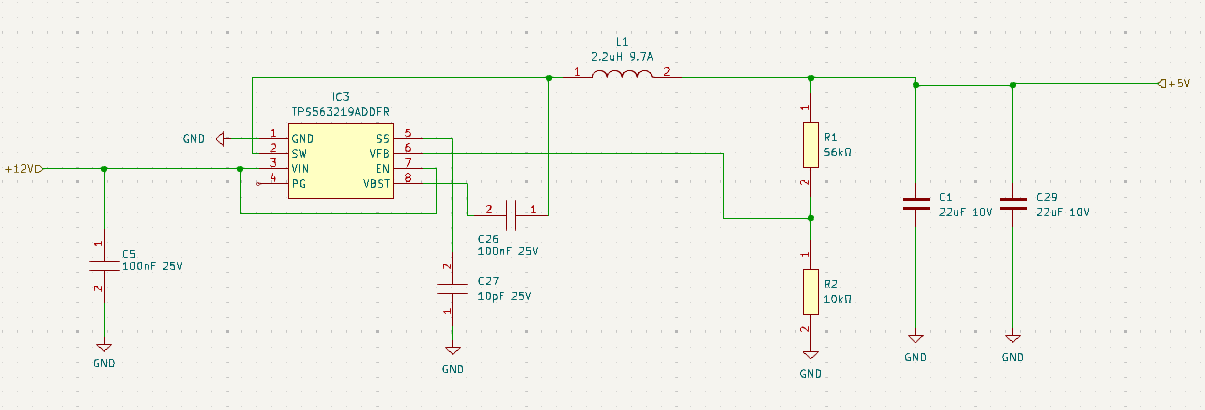
\includegraphics[width=1\textwidth]{5vTo12V_ schemat.png}
    \caption{Schemat złącza DC-Plug}
\end{figure}

\end{document}
